

\section{Äquivalenzrelation von Nerode}
\subsection{Äquivalenzklassen, Faktormenge}
\begin{frame}{Wiederholung}
	\begin{Definition}
		Sei $R \subset A \times A$ eine (binäre) Relation auf der Menge $A$. Wir nennen $R$
		\begin{itemize}
			\item \textbf{reflexiv} falls gilt $$\forall x \in A: (x,x) \in R$$
			\item \textbf{transitiv} falls gilt $$\forall x,y,z \in A: (x,y) \in R \text{ und } (y,z) \in R \implies (x,z) \in R$$
			\item \textbf{symmetrisch} falls gilt $$\forall x,y \in A: (x,y) \in R \implies (y,x) \in R$$
		\end{itemize}
	\end{Definition}
\end{frame}
\begin{frame}{Äquivalenz\dots}
	\begin{Definition}
		Eine Relation $R$ nennt man \textbf{Äquivalenzrelation} wenn sie folgende Eigenschaften erfüllt:
		\begin{itemize}
			\item symmetrisch
			\item reflexiv
			\item transitiv
		\end{itemize}
	\end{Definition}
	\pause
	\begin{Definition}
		Sind zwei Elemente $(x,y) \in R$, so schreibt man auch $xRy$. Alle Elemente, die miteinander in Relation stehen, befinden sich in der selben \textbf{Äquivalenzklasse}: $$[x]_R = \{ y \mid yRx \}$$
	\end{Definition}
\end{frame}

\begin{frame}{Faktormenge}
	\begin{Definition}
		Die Menge aller Äquivalenzklassen einer Menge $M$ zur Relation $R$ bzeichnet man als \textbf{Faktormenge} und schreibt $M_{/R}$.
	\end{Definition}
	\pause
	Zeichnung an der Tafel!
\end{frame}

\begin{frame}{Beweisen Sie...}
	\begin{itemize}
		\item Aus $xRy$ folgt $[x]_R = [y]_R$
		\item Existiert ein $z \in [x]_R$ und $z \in [y]_R$, so ist $[x]_R = [y]_R$
		\item Zu $R = \textbf{mod} \ 6$ gibt es 6 Äquivalenzklassen.
	\end{itemize}
\end{frame}

\begin{frame}{Nerode-Äquivalenzrelation}
	\begin{Definition}
		Sei $L \subseteq A^\ast$ eine formale Sprache. Definiere für zwei Wörter $w_1, w_2 \in A^\ast$: $$w_1 \equiv_L w_2 \iff (\forall w \in A^\ast: w_1 w \in L \iff w_2 w \in L)$$
		Die Relation $\equiv_L$ nennt man \textbf{Äquivalenzrelation von Nerode}
	\end{Definition} \pause
	Äh, hä?
\end{frame}

\begin{frame}{Ein Beispiel}
	Sei $L \subset A^\ast$ die Sprache der Wörter, die das Teilwort $\mathtt{ba}$ nicht enthalten. \pause
	$$L = \langle \mathtt a\ast \mathtt b\ast \rangle$$ Wie sieht ein endlicher Automat dazu aus? \pause 
	\begin{minipage}{0.49\linewidth}\vspace*{1em}
		\centering
		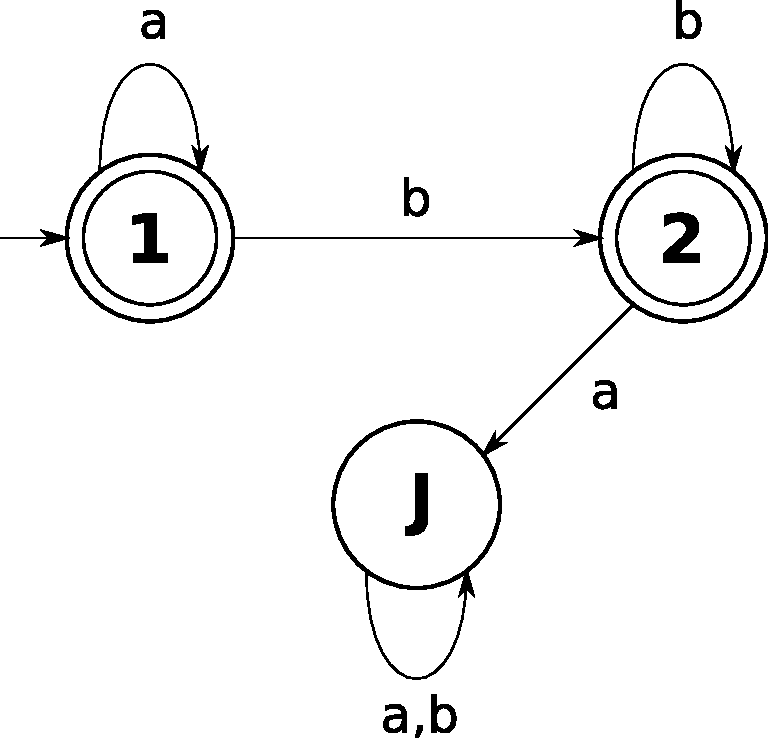
\includegraphics[width=0.8\linewidth]{Nerode.pdf}
	\end{minipage}
	\begin{minipage}{0.49\linewidth}
		Was sind die Nerode Äquivalenz\-klassen? \pause
		Wie komme ich in Zustand 1, 2, J? \pause
		$$\mathtt a^\ast, \mathtt a^\ast \mathtt b \mathtt b^\ast, \mathtt a^\ast \mathtt b \mathtt b^\ast \mathtt a \{\mathtt a, \mathtt b\}^\ast $$ \pause
		Wähle Vertreter! $$[\varepsilon], [\mathtt b], [\mathtt{ba}]$$
	\end{minipage}
\end{frame}

\begin{frame}{Noch ein Beispiel}
	Sei $L \subset A^\ast$ die Sprache 
	$$L = \{ \mathtt a^n \mathtt b \mathtt a^n \mid n \in \N\}$$ Wie sieht ein endlicher Automat dazu aus? \pause
	\begin{minipage}{0.49\linewidth}\vspace*{8em}
		\centering \vfill
		Argh! Es gibt keinen! \vspace*{4em}
	\end{minipage}\pause
	\begin{minipage}{0.49\linewidth}
		Was sind die Nerode Äquivalenz\-klassen? \pause
		Was passiert bei
		\begin{itemize}[<+->]
			\item $\mathtt a^i, i \in \N$
			\item $\mathtt a^i \mathtt b, i \in \N$
			\item dem Rest
		\end{itemize} \pause
		$$\{[\mathtt a^i] \mid i \in \N\} \cup \{[\mathtt a^i \mathtt b] \mid i \in \N\} \cup [\mathtt{ba}]$$
		
	\end{minipage}
\end{frame}


